\documentclass[a4paper,12pt]{article}
\usepackage{graphicx}
\usepackage{hyperref}
\usepackage{amsmath}
\usepackage{times}
\usepackage{xcolor}
\usepackage{amsfonts}
\usepackage{garamondx}
\usepackage{framed}  %This is to use the shaded environment
\usepackage{titlesec}
\usepackage{upquote}



\titlespacing*{\section}
{0pt}{5.5ex plus 1ex minus .2ex}{4.3ex plus .2ex}
\titlespacing*{\subsection}
{0pt}{5.5ex plus 1ex minus .2ex}{4.3ex plus .2ex}

\usepackage{titling}
\setlength{\droptitle}{-8em} 


\textwidth=6.2in
\textheight=8.5in
%\parskip=.3cm
\oddsidemargin=.1in
\evensidemargin=.1in
\headheight=-.3in
\setlength{\parindent}{0pt}



% \renewcommand{\baselinestretch}{1} 
% \setlength{\parskip}{\baselineskip}
% \setlength{\parindent}{0pt}
% \setlength{\marginparwidth}{2.5cm}


\newcommand{\scscst}{\scriptscriptstyle}
\newcommand{\scst}{\scriptstyle}
\newcommand{\Robject}[1]{{\code{#1}}}
\newcommand{\Rfunction}[1]{{\code{#1}}}
\newcommand{\Rclass}[1]{\textit{#1}}
\newcommand{\Rpackage}[1]{\textit{#1}}
\newcommand{\Rexpression}[1]{\code{#1}}
\newcommand{\Rmethod}[1]{{\code{#1}}}
\newcommand{\Rfunarg}[1]{{\code{#1}}}

\newcommand\boldblue[1]{\textcolor{blue}{\textbf{#1}}}
\newcommand\code[1]{\textcolor{red}{\texttt{#1}}}

\usepackage{Sweave}
\begin{document}
\Sconcordance{concordance:1_Stats_Course_Notes-knitr.tex:1_Stats_Course_Notes-knitr.Rnw:%
1 50 1 1 0 5 1 1 7 13 1 1 9 1 1 1 7 160 1 1 5 9 0 1 2 5 1 1 2 1 0 2 1 %
13 0 1 2 8 1 1 2 1 0 1 3 4 0 1 2 3 1 1 4 1 1 1 4 7 0 1 2 8 1}

\definecolor{shadecolor}{gray}{0.95} %this is defining the color of the background in the shaded environment

%\SweaveOpts{concordance=TRUE}



%------------------------------------------------------------
\title{Using R as a Research Tool.\\
Part 2: R Markdown and Basic Statistics.}
%------------------------------------------------------------
\author{Dr Susan Johnston: \href{mailto:Susan.Johnston@ed.ac.uk}{Susan.Johnston@ed.ac.uk}  \\ \\
Demonstrators \& Contributors: Gergana Daskalova, John Godlee. \\
Hat-Tips to Kyle Dexter, The Coding Club and R4all.}
\date{}






\maketitle

%\tableofcontents

\vspace*{-2.5cm}.
%-------------------------------------------
\section {Introduction}
%-------------------------------------------

This practical will follow on from the previous practical in data manipulation and visualisation, exploring how to write reports in \boldblue{R} Markdown and how to conduct simple statistical tests in \boldblue{R}. By the end of the practical, you should be able to:

\begin{itemize}

\item Write, embed and render code and results into an HTML document.

\item Carry out basic statistics and visualisations, including:

\begin{itemize}

\item Chi-squared ($\chi^{2}$) test with \code{chisq.test()}
\item 2-sample t-test with \code{t.test()}
\item Linear regression with \code{lm()}


\end{itemize}

\end{itemize}



%-------------------------------------------
\section {Writing reports with R Markdown.}
%-------------------------------------------


\boldblue{R} Markdown is a tool for writing reproducible reports in \boldblue{R}. It can be used to produce documents with embedded code and figures in HTML, Word and PDF format, and can also be used to create webpages and slideshows. The  \boldblue{R} Markdown Cheatsheet from RStudio is included in the github repository \url{https://github.com/susjoh/Intro_to_Stats_in_R}.

\subsection{Creating an R Markdown Document.}

Open RStudio and create a new markdown document by going to \textbf{File > New File > R Markdown...}. In the window, name your document, select \textbf{HTML} and click \textbf{OK}. RStudio should automatically create a template as in Figure \ref{fig:MarkdownTemplate} (if not - it is saved in the file \texttt{R\_Markdown\_Template.Rmd)}. \\

To render the document, click the button that says \code{Knit} (you may have to save it first). As you can see, it produces a formatted HTML document with embedded figures that reflect the text and code within the markdown file. Take some time to familiarise yourself with how the script matches to the output. \\

A convenient feature of \boldblue{R} Markdown in RStudio is the \textbf{Show document outline} in the top right corner of the window. For very long scripts, adding \verb!####! or \verb!----! to a comment line will include that comment in the document outline. Try it out. It is possible to carry out basic formatting as well as adding headings, tables, lists and external figures. See Part 3 of the \boldblue{R} Markdown CheatSheet. \\

\begin{figure}[h]
\centering 
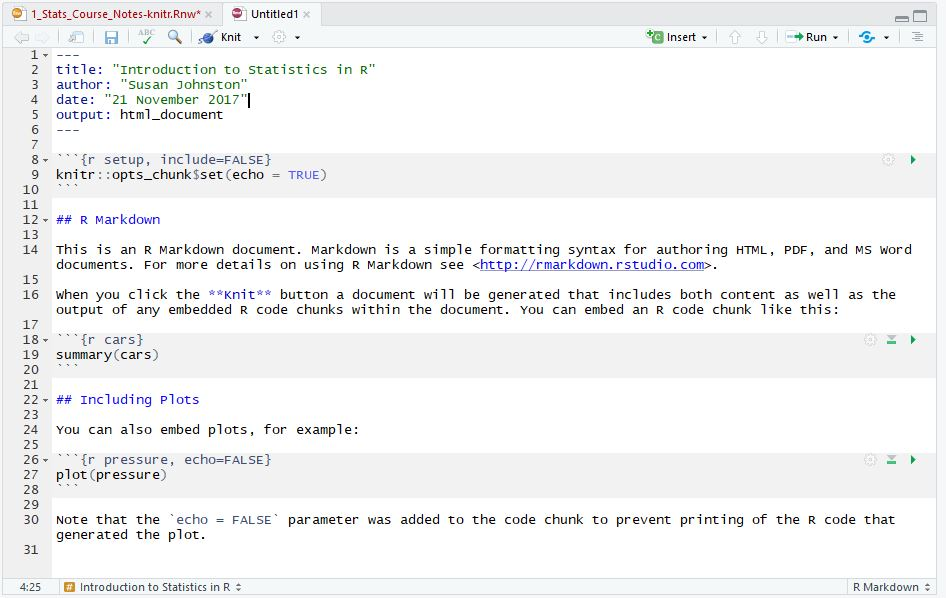
\includegraphics[width=0.8\textwidth]{figs/MarkdownTemplate.JPG}
\caption{R Markdown Template.}
\label{fig:MarkdownTemplate}
\end{figure} 


\fbox{\begin{minipage}{36em}
\Large{\textbf{Exercise 1.}}

\normalsize
1. Create a new \boldblue{R} Markdown Script with the following header:\\


\texttt{---}\\
\texttt{title:} ``\texttt{Introduction to Statistics in R}''\\
\texttt{author:} ``\texttt{Your Name}''\\
\texttt{date:} ``\texttt{28 November 2017}'' \\
\texttt{output: html\_document} \\
\texttt{---} \\


Add some text \& familiarise yourself with basic formatting (e.g. \textit{italic}, \textbf{bold}). Add headers for ``Introduction'', ``Chi-square test'',  ``Two-sample t-test`` and ``Linear regression''.
\end{minipage}}


\subsection{Embedding code in R Markdown.}

Code can be embedded into the document in two ways: \\

\textbf{Code Chunks:}
\begin{shaded}
\begin{verbatim}
```{r}
head(iris)
```
\end{verbatim}
\end{shaded}

Code chunks can be named, e.g. \verb!```{r iris}! \\

\textbf{Inline code:}
\begin{shaded}
\begin{verbatim}
Two plus two equals `r 2 + 2`.
\end{verbatim}
\end{shaded}

Which will print ``Two plus two equals 4.''.

\vspace*{-1cm}.

\subsection{Structuring an R Markdown document.}

As you have seen in the example, there can be several code chunks within a document. Each chunk is run sequentially and saved in the working environment. Therefore libraries and new objects created in a chunk will remain in the workspace for all subsequent chunks. When clicking ``\code{Knit}'', RStudio will assume that the directory containing the file is the working directory. \\

The first chunk in your Markdown document is a good place to load libraries and data. In this practical, we will use the libraries \code{ggplot2} and \code{dplyr}. Put this chunk after the header of your document and click \code{Knit}:

\begin{shaded}
\begin{verbatim}
```{r}
library(ggplot2)
library(dplyr)
```
\end{verbatim}
\end{shaded}

You may notice that this results in some unsightly code that is not relevant to the document. It is possible to control what is reported in the document using additional markers within the chunk description. For example, the following will allow the command to run invisibly:

\begin{shaded}
\begin{verbatim}
```{r echo = FALSE, message = FALSE, warning = FALSE}
library(ggplot2)
library(dplyr)
```
\end{verbatim}
\end{shaded}

It can also control how results and figures are presented. Try \code{knit}ting:

\begin{shaded}
\begin{verbatim}
```{r}
data(iris)
str(iris)
ggplot(iris, aes(x = Sepal.Length, y = Sepal.Width)) + geom_point()
```
\end{verbatim}
\end{shaded}

and then replacing it with the following, and \code{knit}ting again:

\begin{shaded}
\begin{verbatim}
```{r echo = F, results = "hide", fig.width = 4, fig.height = 3}
data(iris)
str(iris)
ggplot(iris, aes(x = Sepal.Length, y = Sepal.Width)) + geom_point()
```
\end{verbatim}
\end{shaded}

The second option will hide the code (\texttt{echo = F}) and code output (\texttt{results = "hide"}) but show the figure (dimensions specified with \texttt{fig.width} and \texttt{fig.height}). A full list of options are given in Figure \ref{fig:markdownrules}.

\begin{figure}[h]
\centering 
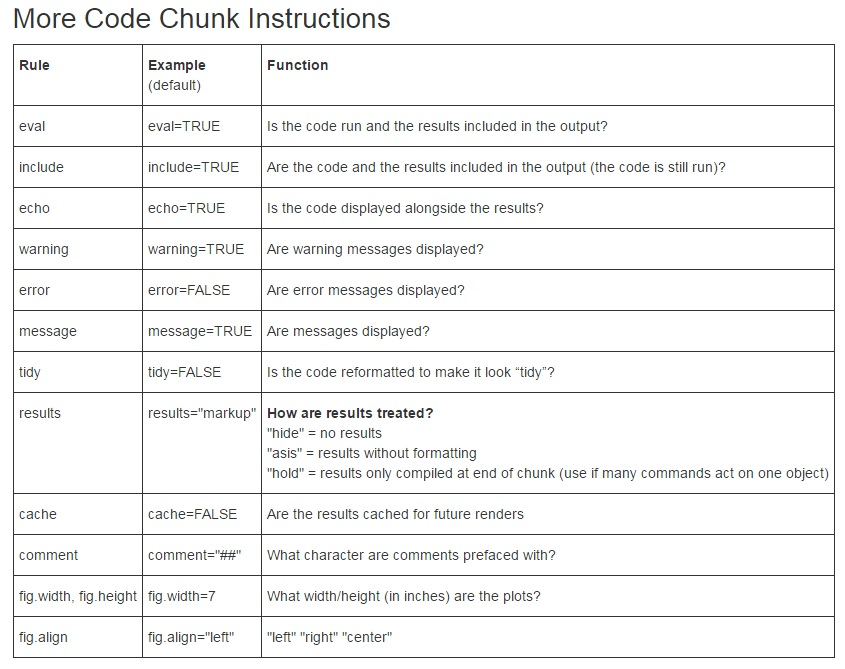
\includegraphics[width=1\textwidth]{figs/markdownrules.jpg}
\caption{R Markdown Code Instrucutions.}
\label{fig:markdownrules}
\end{figure} 


\subsection{Important Points to Note.}

\begin{itemize}

\item Code in \boldblue{R} Markdown chunks can be run in the console as in the previous practical. The default option is to show the code output inline in the document. Some people like this, others don't: to switch this function on and off, go to \textbf{Global options > R Markdown >Show output inline for all Markdown documents} and select your preferred setup.

\item \boldblue{R} Markdown documents are not flexible to errors - the code must be error free, or it will not render.

\item Want to learn more? More detailed information on this can be found at the Coding Club tutorial at \url{https://ourcodingclub.github.io/2016/11/24/rmarkdown-1.html}. \\

\end{itemize}




%-------------------------------------------
\section{Basic statistics.}
%-------------------------------------------

\textbf{For the rest of the practical, it is expected that you create an R Markdown document that contains text, code, graphs and inline reporting of results.} We will approach this using the  approach of examining the data through visualisation, form our hypothesis, carry out the statistical test and then \code{Knit} this information into our document. \\


\begin{figure}[h]
\centering 
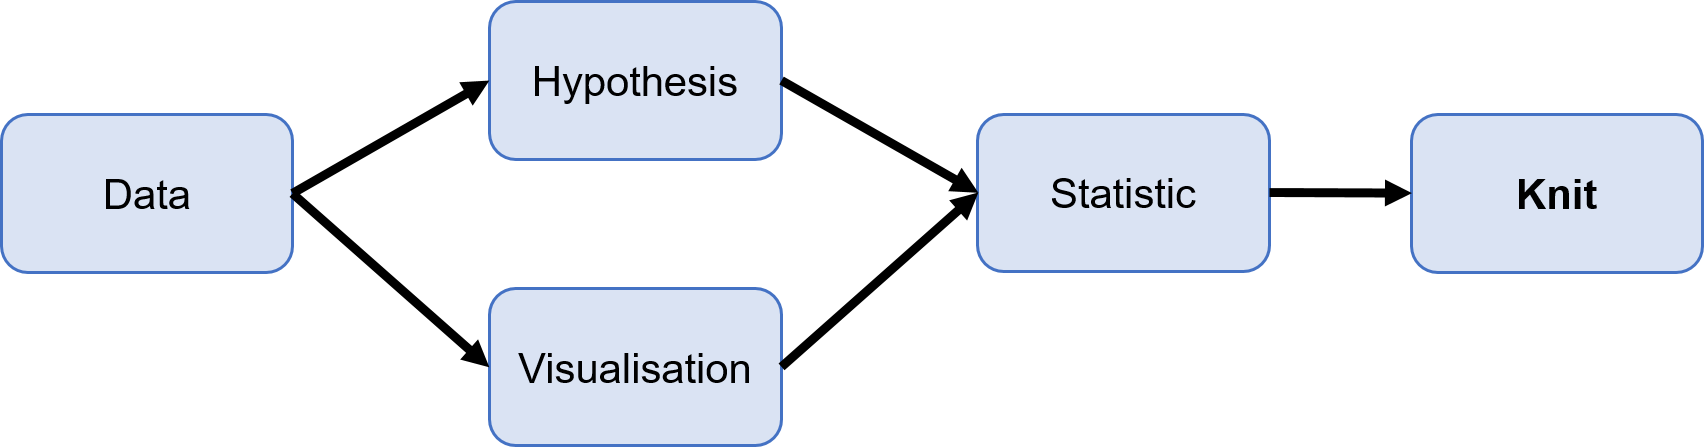
\includegraphics[width=.8\textwidth]{figs/StatisticsFlow2.png}
\label{fig:StatisticsFlow}
\end{figure} 

In the interests of time, this practical will focus on the \textbf{how} rather than \textbf{why} we will do these tests. We highly recommend doing further reading in your own time, such as ``Getting Started with R'' (2nd Edition, 2017) by Beckerman, Childs and Petchey (\url{http://www.r4all.org}). Let's begin!



%-------------------------------------------
\section{Chi-squared ($\chi^{2}$) contingency table}
%-------------------------------------------

A $\chi ^{2}$ contingency table analyses count data, and looks at the association between two or more categorical variables. In this example, we will examine the differences in the frequency of red and black ladybirds (\textit{Adalia bipunctata}) in rural and industrial habitats. Our question is: are dark morphs more likely to reside in dark (industrial) backgrounds? The null hypothesis is that there is no association between ladybird colour morph and habitat type \footnote{The approach and dataset here is based on the example presented in the book ``Getting Started with R'' (2nd Edition, 2017) by Beckerman, Childs and Petchey (\url{http://www.r4all.org})}. \\

Load the data file \texttt{ladybirds.csv} into R using \code{read.csv()} and examine it using \code{glimpse()} from the \code{dplyr} package.

\begin{shaded}
\begin{verbatim}
library(dplyr)

ladybirds <- read.csv("data/ladybirds.csv", header = T)
glimpse(ladybirds)
\end{verbatim}
\end{shaded}

\begin{Schunk}
\begin{Soutput}
Observations: 20
Variables: 4
$ Habitat      <fctr> Rural, Rural, Rural, Rural, Rural, Rural, Rural, Rura...
$ Site         <fctr> R1, R2, R3, R4, R5, R1, R2, R3, R4, R5, U1, U2, U3, U...
$ morph_colour <fctr> black, black, black, black, black, red, red, red, red...
$ number       <int> 10, 3, 4, 7, 6, 15, 18, 9, 12, 16, 32, 25, 25, 17, 16,...
\end{Soutput}
\end{Schunk}

There are multiple lines for each category, with the column number giving the count details. We ultimately want four numbers, corresponding to the 2 $\times$ 2 categories: \underline{red industrial}, \underline{black industrial}, \underline{red rural} and \underline{black rural}. \\

This can be done using the \code{dplyr} functions \code{group\_by()} amd \code{summarise()}.

\begin{shaded}
\begin{Schunk}
\begin{Sinput}
> totals <- group_by(ladybirds, Habitat, morph_colour)
> totals <- summarise(totals, total.number = sum(number))
> totals
\end{Sinput}
\begin{Soutput}
# A tibble: 4 x 3
# Groups:   Habitat [?]
     Habitat morph_colour total.number
      <fctr>       <fctr>        <int>
1 Industrial        black          115
2 Industrial          red           85
3      Rural        black           30
4      Rural          red           70
\end{Soutput}
\end{Schunk}
\end{shaded}

\subsection{Plot the data}

One visualisation for this type of data is a bar chart using \code{geom\_col()} in \code{ggplot2}.


\begin{shaded}
\begin{Schunk}
\begin{Sinput}
> library(ggplot2)
> ggplot(totals, aes(x = Habitat, y = total.number, fill = morph_colour)) +
+   geom_col() 
\end{Sinput}
\end{Schunk}
\end{shaded}

There are two edits we can make to this to improve the visualisation: to add \code{geom\_col(position = "dodge")} to place bars side by side, and to use \code{scale\_fill\_manual()} to change the colours of the bars to black and red to match the colour of the morphs in real life:


\begin{shaded}
\begin{Schunk}
\begin{Sinput}
> ggplot(totals, aes(x = Habitat, y = total.number, fill = morph_colour)) +
+   geom_col(position = "dodge") +
+   scale_fill_manual(values = c(black = "black", red = "red"))
\end{Sinput}
\end{Schunk}
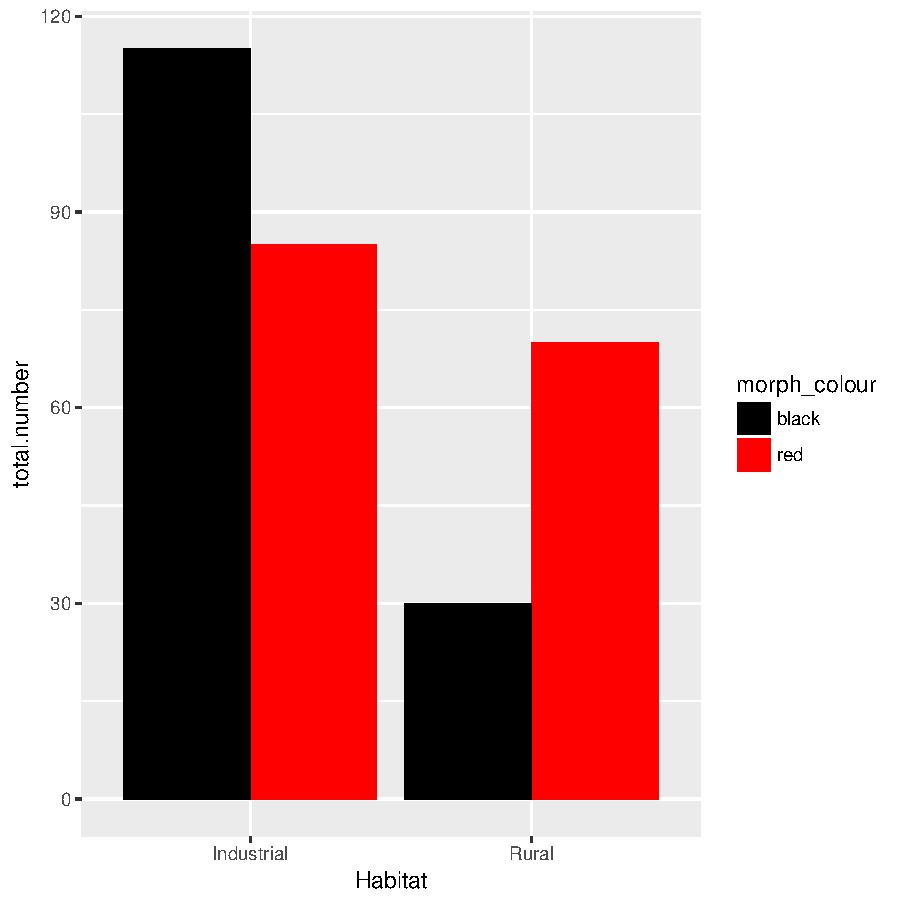
\includegraphics{1_Stats_Course_Notes-knitr-008}
\end{shaded}

\subsection{Test the hypothesis with \code{chisq.test()}.}

The $\chi^{2}$ is run using the function \code{chisq.test()}. As this is a 2 $\times$ 2 contingency test, we must convert the data into a matrix. Looking at the data \code{ladybirds}, a matrix can be made using the function \code{xtabs()}, which is similar to creating pivot table cross-tabulation in Excel:

\begin{shaded}
\begin{Schunk}
\begin{Sinput}
> lady.mat <- xtabs(number ~ Habitat + morph_colour, data = ladybirds)
> lady.mat
\end{Sinput}
\begin{Soutput}
            morph_colour
Habitat      black red
  Industrial   115  85
  Rural         30  70
\end{Soutput}
\end{Schunk}
\end{shaded}

Now run the test:

\begin{shaded}
\begin{Schunk}
\begin{Sinput}
> chisq.test(lady.mat)
\end{Sinput}
\begin{Soutput}
	Pearson's Chi-squared test with Yates' continuity correction

data:  lady.mat
X-squared = 19.103, df = 1, p-value = 1.239e-05
\end{Soutput}
\end{Schunk}
\end{shaded}


This provides a statistic indicating that there is a very small probability that the observed pattern arose by chance. Therefore, we can reject the null hypothesis. We can extract more information from the statistic if we save the \code{chisq.test(ladymat)} as an object:

\begin{shaded}
\begin{Schunk}
\begin{Sinput}
> lady.chisq <- chisq.test(lady.mat)
\end{Sinput}
\end{Schunk}
\end{shaded}

Running \code{lady.chisq} gives the same output as before, but we can explore the object in detail using the \code{\$} notation:

\begin{shaded}
\begin{Schunk}
\begin{Sinput}
> names(lady.chisq)
\end{Sinput}
\begin{Soutput}
[1] "statistic" "parameter" "p.value"   "method"    "data.name" "observed" 
[7] "expected"  "residuals" "stdres"   
\end{Soutput}
\begin{Sinput}
> # str(lady.chisq) # not run here to save space - please run it!
> 
> lady.chisq$statistic
\end{Sinput}
\begin{Soutput}
X-squared 
 19.10289 
\end{Soutput}
\begin{Sinput}
> lady.chisq$p.value
\end{Sinput}
\begin{Soutput}
[1] 1.238571e-05
\end{Soutput}
\end{Schunk}
\end{shaded}

In the \boldblue{R} Markdown document, it is possible to quote statistics inline using the \verb!`r`! notation e.g. \verb!`r lady.chisq$statistic`! and \verb!`r lady.chisq$p.value`! will print the $\chi^{2}$ statistic and P value inline, respectively. \\


\fbox{\begin{minipage}{36em}
\Large{\textbf{Exercise 2.}}

\normalsize 
Create a short report in the \boldblue{R} Markdown document with an inline report of the test statistics and P-value. This can be done as follows:
\begin{enumerate}
\item Add a code chunk for loading and manipulating the data, and running the $\chi^{2}$ test.
\item Edit the previous chunk options so that it does \textbf{not} print the code or results to the compiled document (hint: define \code{echo} and \code{results} in the chunk options).
\item Write a few lines of text stating the hypothesis, the test statistic and interpretation. E.g.\\ \textit{The null hypothesis is... Ladybird morphs are not equally distributed in the two habitats (Chi squared = ..., df = ..., P = ...), with black morphs being more frequent in the ... habitat.}
\item Add a code chunk to output the figure that illustrates the results of the $\chi^{2}$ test.
\end{enumerate}

\end{minipage}}

%-------------------------------------------
\section{Two-sample t-test.}
%-------------------------------------------

A two-sample t-test is one of the most conceptually simple and commonly used hypothesis tests. It determines whether the mean of two groups of numeric values are significantly different from each other, or are due to random chance. Here, we will use data from two \textit{Iris} species, \textit{I. virginica} and \textit{I. versicolor} to determine if their Sepal lengths are significantly different (Figure \ref{fig:IrisVirginica}). \\

\begin{figure}[h]
\centering 
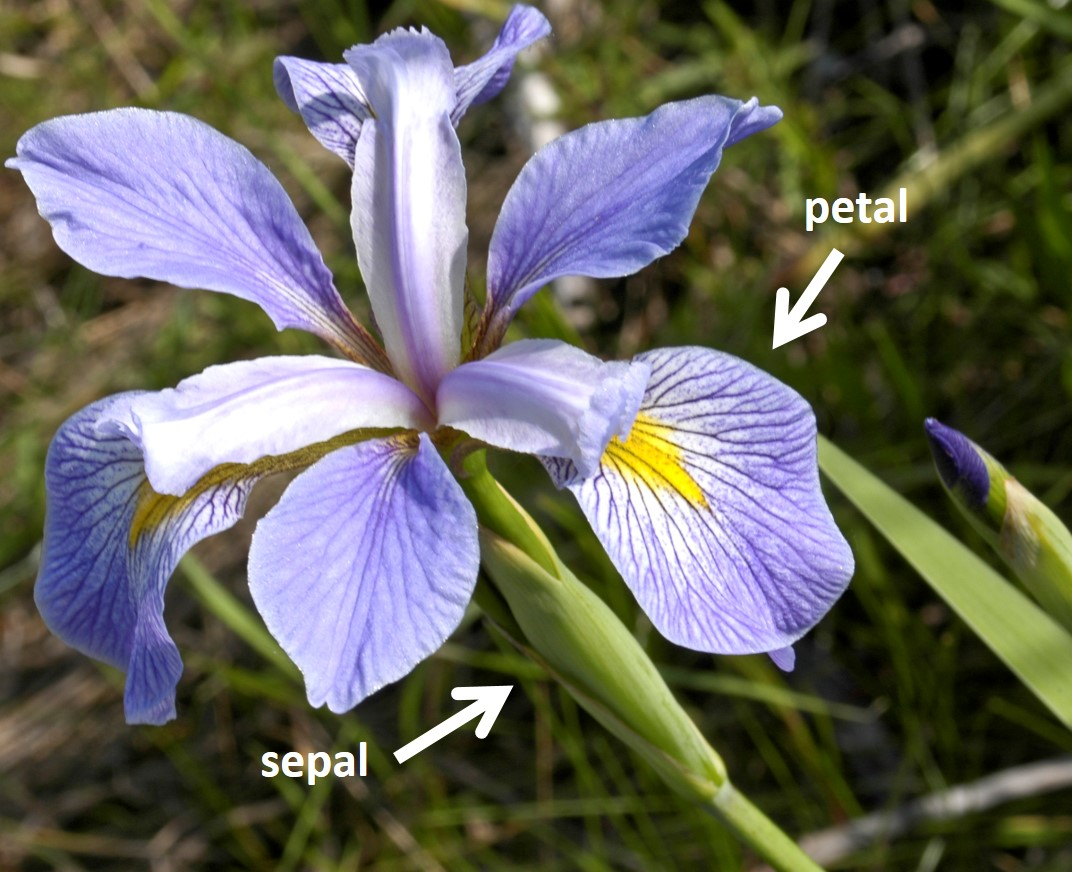
\includegraphics[width=0.5\textwidth]{figs/Irisvirginica.jpg}
\caption{\textit{Iris virginica.}}
\label{fig:IrisVirginica}
\end{figure} 

This test makes two assumptions about the data - that both groups are normally distributed and that the variances are equal in each category. For the interests of time, we will assume that both of these assumptions are met\footnote{These assumptions can be tested using \code{shapiro.test()} and \code{var.test()} on specific specific value vectors. If you would like to try this and need help, use the \code{?} command or ask the demonstrators.}.\\

First, load the data:

\begin{shaded}
\begin{verbatim}
sepals <- read.csv("../data/iris.edited.csv", header = T)
glimpse(sepals)
\end{verbatim}


\begin{Schunk}
\begin{Soutput}
Observations: 100
Variables: 2
$ Species      <fctr> versicolor, versicolor, versicolor, versicolor, versi...
$ Sepal.Length <dbl> 7.0, 6.4, 6.9, 5.5, 6.5, 5.7, 6.3, 4.9, 6.6, 5.2, 5.0,...
\end{Soutput}
\end{Schunk}
\end{shaded}


The first step is to visualise the data. One approach is to use a boxplot, which is more visually appealing (but based on the median rather than the mean) - another is to use histograms. These can help us to assess if the means seem different between the two categories, and if the data is normally distributed with a similar variance. It can also provide an inidication of whether the null hypothesis can be accepted or rejected.

\begin{shaded}
\begin{verbatim}
# boxplot

ggplot(sepals, aes(Species, Sepal.Length)) + geom_boxplot()

# histogram with facet_wrap

ggplot(sepals, aes(Sepal.Length)) + 
geom_histogram(binwidth = 0.25) + 
facet_wrap(~Species, ncol = 1)
\end{verbatim}
\end{shaded}

\begin{figure}[h]
\centering 
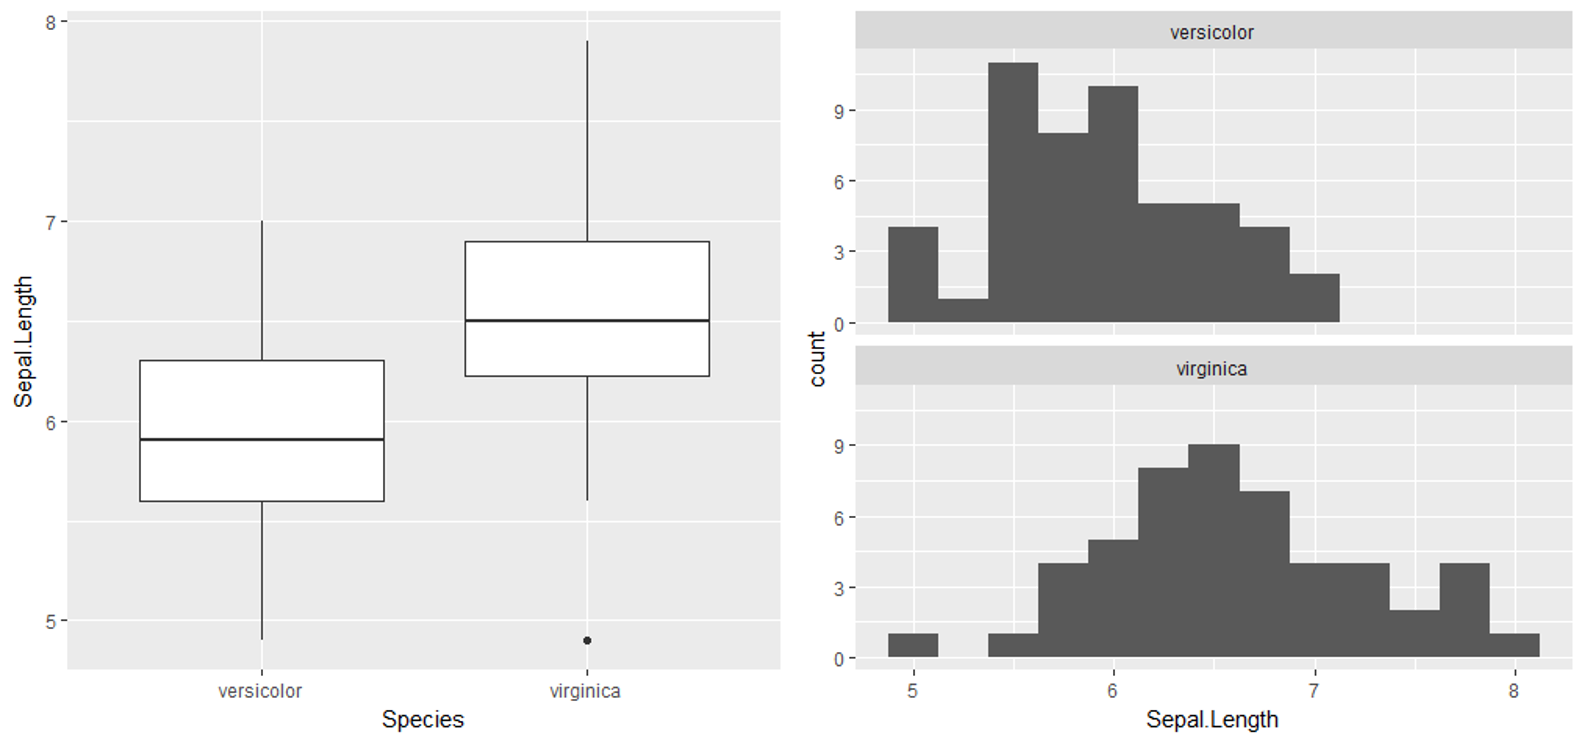
\includegraphics[width=1\textwidth]{figs/boxplothist.png}
\label{fig:boxplothist}
\end{figure} 


To carry out the t-test, we will use the \code{t.test()} function. We can find out the details of the test using \code{?t.test}. The syntax requires a formula \code{Sepal.Length $\sim$ Species} and the data frame (\code{data = sepals}). This should reflect the hypothesis - how does sepal length vary as a function of species? \\


\begin{shaded}
\begin{Schunk}
\begin{Sinput}
> sepal.test <- t.test(Sepal.Length ~ Species, data = sepals)
> sepal.test
\end{Sinput}
\begin{Soutput}
	Welch Two Sample t-test

data:  Sepal.Length by Species
t = -5.6292, df = 94.025, p-value = 1.866e-07
alternative hypothesis: true difference in means is not equal to 0
95 percent confidence interval:
 -0.8819731 -0.4220269
sample estimates:
mean in group versicolor  mean in group virginica 
                   5.936                    6.588 
\end{Soutput}
\end{Schunk}
\end{shaded}

The function has automatically used the Welch version of the t-test, which relaxes the assumption of equal variances - this is fine for the purposes of this practical (see Beckerman et al for a discussion of this in more detail). The output provides the \code{t}, \code{df} and \code{p-value} for the test, as well as the mean value in each of the two groups. The 95\% confidence interval shows the interval between the difference between the two means - if this overlapped 0, then we would retain the null hypothesis.\\

Therefore, given the output, we can reject the null hypothesis, and can conclude that \textit{I. virginica} has longer sepals than \textit{I. versicolor}.


\fbox{\begin{minipage}{36em}
\Large{\textbf{Exercise 3.}}\\

\normalsize 

1. Create a short report in the \boldblue{R} Markdown document with an inline report as for Exercise
2.\\

2. Use the Cheat Sheet (Hint: Section 3) to add the image of \textit{Iris virginica} to the Markdown document (``\texttt{data/Irisvirginica.jpg}'')

\end{minipage}}


%-------------------------------------------
\section{Simple Linear regression.}
%-------------------------------------------

The last model we will tackle is a linear regression. This is the most basic of a class of models called `\textbf{general linear models}' which also includes multiple regression and ANOVA. \\

For this, we will use one of the first datasets upon which linear regression was performed, which is Francis Galton's human height dataset from 1886 \footnote{Whilst Francis Galton made many important contributions to statistics, geosciences, genetics and psychology, like Ronald Fisher, he was also a keen eugenicist. The data is presented here as a historical scientific spirit, and in no way condones his views.}. This dataset contains information on mother and father heights, as well as the height and sex of their adult children. \\

The data can be called as follows:

\begin{shaded}
\begin{verbatim}
heights <- read.csv("data/Galton.csv", header = T)
head(heights)
\end{verbatim}
\begin{Schunk}
\begin{Soutput}
  family father mother sex height nkids mid.parent
1      1   78.5   67.0   M   73.2     4      72.75
2      1   78.5   67.0   F   69.2     4      72.75
3      1   78.5   67.0   F   69.0     4      72.75
4      1   78.5   67.0   F   69.0     4      72.75
5      2   75.5   66.5   M   73.5     4      71.00
6      2   75.5   66.5   M   72.5     4      71.00
\end{Soutput}
\end{Schunk}
\begin{Schunk}
\begin{Sinput}
> dim(heights)
\end{Sinput}
\begin{Soutput}
[1] 898   7
\end{Soutput}
\end{Schunk}
\end{shaded}


There are a number of columns here, including identifiers for the family and the number of children. We will focus on \code{height} (the adult child height in inches) and \code{mid.parent} (the mid-parental height between the mother and father). As there is a strong sex difference in child height, we will filter the dataset to only include female offspring.

\begin{shaded}
\begin{Schunk}
\begin{Sinput}
> heights <- filter(heights, sex == "F")
> dim(heights)
\end{Sinput}
\begin{Soutput}
[1] 433   7
\end{Soutput}
\end{Schunk}
\end{shaded}

Our question is whether offspring height varies relative to the mean height of their parents. Here, offspring height is the response (dependent) variable, whereas mid-parental height is the explanatory (independent) variable. Both are continuous, numeric variables. \\

Visualise the data:

\begin{shaded}
\begin{Schunk}
\begin{Sinput}
> ggplot(heights, aes(x = mid.parent, y = height)) + 
+   geom_point() +
+   labs(x = "Mid-parental height", y = "Daughter height")
\end{Sinput}
\end{Schunk}
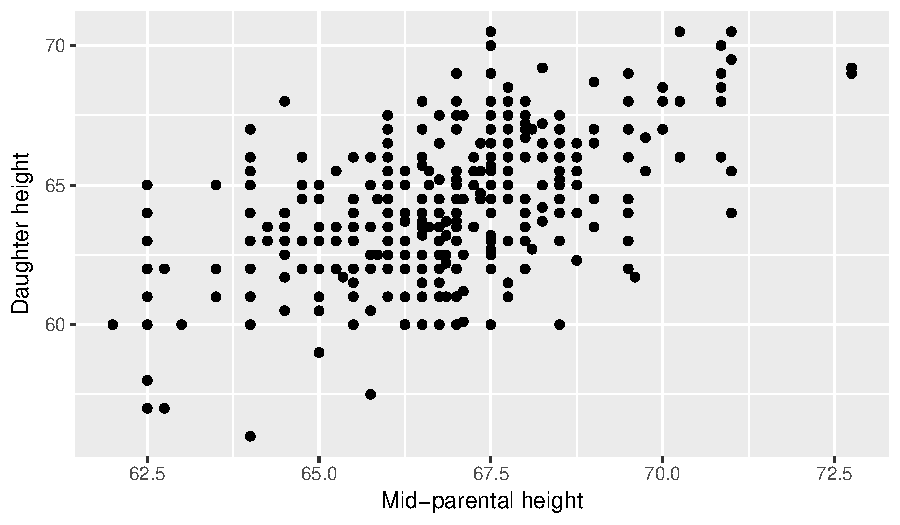
\includegraphics{1_Stats_Course_Notes-knitr-018}
\end{shaded}

Visually, it looks like there is a positive relationship between mid-parental height and daughter height - taller parents have taller daughters. We can test this using the function \code{lm()} to fit the model. The syntax is similar to that of the t-test above:

\begin{shaded}
\begin{Schunk}
\begin{Sinput}
> lm.heights <- lm(height ~ mid.parent, data = heights)
\end{Sinput}
\end{Schunk}
\end{shaded}

Before examining the output, it is important to check the assumptions of the linear model. This can be done using the \code{autoplot()} function in \code{library(ggfortify)} to examine the model residuals: \footnote{You may need to install this package using \code{install.packages("ggfortify")}.} \\

\begin{shaded}
\begin{Schunk}
\begin{Sinput}
> library(ggfortify)
> autoplot(lm.heights)
\end{Sinput}
\end{Schunk}
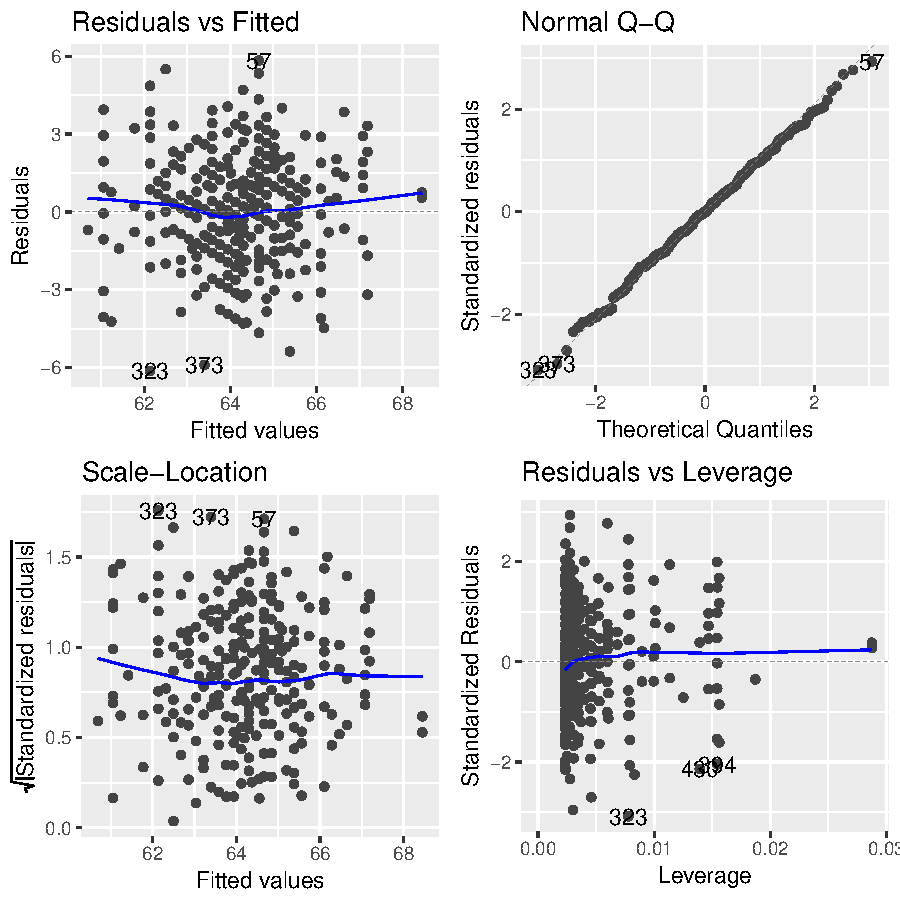
\includegraphics{1_Stats_Course_Notes-knitr-020}
\end{shaded}

Generally these plots look good - although we have limited time to understand them in detail, we can quickly intepret them as follows:

\begin{itemize}
\item The \textbf{top left} plot determines if the line is an appropiate fit to the data. A relatively straight line is good - something humped would indicate that a non-linear relationship. 
\item The \textbf{top right} plot shows if the residuals are normally distributed - they should line up on the straight dashed line.
\item The \textbf{bottom left} plot is a check of equal variances; again, a lack of pattern (i.e. a horizontal line) shows the model is an appropriate fit.
\item Finally, the \textbf{bottom right} panel shows the residuals vs. leverage, to determine some of the data points have a particularly strong influence on the regression line. A straight line and all data within the Cook's distance lines (these do not appear in this plot) indicate that this is not an issue in the data.
\end{itemize}

Given that the data looks good, let's examine the output form the statistical model:

\begin{shaded}
\begin{Schunk}
\begin{Sinput}
> lm.heights
\end{Sinput}
\begin{Soutput}
Call:
lm(formula = height ~ mid.parent, data = heights)

Coefficients:
(Intercept)   mid.parent  
    15.9671       0.7214  
\end{Soutput}
\end{Schunk}
\end{shaded}

As you can see, calling the statistical model alone only provides us with two values - the model intercept and the slope. The slope is positive, and suggests that for for each unit increase in mid-parental height, there is an increase in daughter height by 0.72 inches.\\

However, calling this alone does not provide information on whether we can reject the null hypothesis. For this, we use the \code{summary()} function:

\begin{shaded}
\begin{Schunk}
\begin{Sinput}
> summary(lm.heights)
\end{Sinput}
\begin{Soutput}
Call:
lm(formula = height ~ mid.parent, data = heights)

Residuals:
    Min      1Q  Median      3Q     Max 
-6.1365 -1.3989  0.0028  1.4207  5.8386 

Coefficients:
            Estimate Std. Error t value Pr(>|t|)    
(Intercept) 15.96711    3.60237   4.432 1.18e-05 ***
mid.parent   0.72140    0.05396  13.369  < 2e-16 ***
---
Signif. codes:  0 '***' 0.001 '**' 0.01 '*' 0.05 '.' 0.1 ' ' 1

Residual standard error: 1.995 on 431 degrees of freedom
Multiple R-squared:  0.2931,	Adjusted R-squared:  0.2915 
F-statistic: 178.7 on 1 and 431 DF,  p-value: < 2.2e-16
\end{Soutput}
\end{Schunk}
\end{shaded}

We can see here that the observed positive slope is highly significant (\texttt{\textless 2e-16}). \\

Finally, we can add the slope to the plot using \code{stat\_smooth(method = "lm")}:

\begin{shaded}
\begin{Schunk}
\begin{Sinput}
> ggplot(heights, aes(x = mid.parent, y = height)) + 
+   geom_point() +
+   stat_smooth(method = "lm") +
+   labs(x = "Mid-parental height", y = "Daughter height")
\end{Sinput}
\end{Schunk}
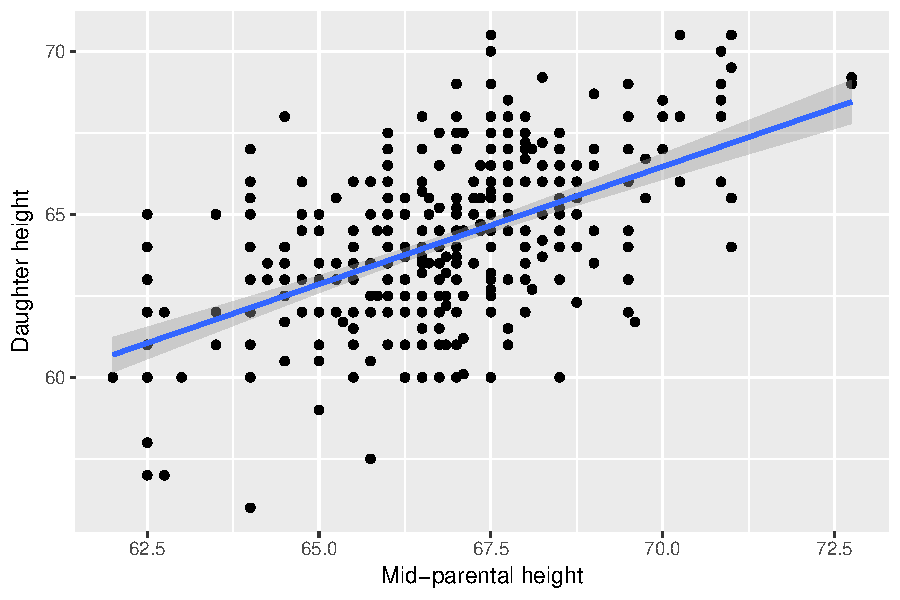
\includegraphics{1_Stats_Course_Notes-knitr-023}
\end{shaded}

\fbox{\begin{minipage}{36em}
\Large{\textbf{Exercise 4.}}\\

\normalsize 

1. Create a short report in the \boldblue{R} Markdown document with an inline report as for Exercises 2 and 3. Remember to report the slope, t-statistic, degrees of freedom and P-value.\\

Hint: extracting values from the model can use indexing as visited in the DataCamp tutorial. The best approach is to create an object for the summary of lm.heights e.g. \code{summary.lm.heights <- summary(lm.heights)\$coefficients} and calling values based on the indices (e.g. the t-value will be \code{summary.lm.heights[2,3]}.
\end{minipage}}





\end{document}

